\section{Реализация}
\subsection{Список используемых технологий}
\begin{enumerate}
\item JavaScript — интерпретируемый браузером язык программирования.
\item HTML5, CSS — языки разметки для создания интерфейса.
\item Bootstrap, jQuery — подключённые библиотеки.
\item LaTeX — система компьютерной верстки, значительно облегчающая создание технической литературы. Используется для создания отчёта.
\item VCS Git — система контроля версий.
\end{enumerate}
\subsection{Язык программирования и библиотеки}
Для реализации поставленных задач был выбран язык JavaScript. Его программой-интерпретатором является браузер (ссылка). Язык прост в освоении, имеет похожий на язык C синтаксис, динамическую типизацию переменных, элементы объектно-ориентированного программирования позволяет работать с обработчиками событий(сслыка).

JavaScript поддерживается всеми современными браузерами, что обеспечивает реализованной программе кроссплатформенность и возможность запуска даже на мобильных устройствах.

По соображениям безопасности, на язык наложены некоторые ограничения. Он не имеет прямого доступа к операционной системе. Например, возможность чтения и записи файлов сильно ограничена.

Язык имеет полную интеграцию с языком разметки HTML и CSS. Первый позволяет создавать прототип интерфейса, его скелет, а второй определяет внешний вид объектов интерфейса.

Вместе тройка данных языков предоставляет невероятные возможности для построения интерфейса и визуализации, что хорошо подходит для осуществления поставленных задач.

Для упрощения работы подключены библиотеки jQuery и Bootstrap. jQuery используется для быстрого доступа к содержимому HTML и необходим для работы Bootstrap. Bootstrap предоставляет готовые решения для элементов интерфейса, выполненные профессиональными дизайнерами. 

Совокупность перечисленных языков и библиотек позволяет сосредоточится на алгоритмах и правильной работе коде, а не тратить время на изучение огромного количества документации к интерфейсу, как в многих решениях для компилируемых языков программирования.
\subsection{Реализации алгоритмов}
\subsubsection{Структура карты}
Граф представлен сеткой (англ. Grid) — массив клеток, который условно можно назвать картой. Каждая клетка является вершиной, имеющей 4 или 8 соседних вершин в зависимости от разрешённости диагонального движения. Координаты клетки определяются её положением в двухмерном массиве карты. Чтобы не загружать браузер вычислениями квадратного корня, вес ребра равен вертикального и горизонтального ребра равны 10, а диагонального 14.

Рассмотрим клетку как прототип объекта. Определены поля $f$, $h$, $g$, $parent$, $closed$, $visited$, $type$, $i$, $j$. Значения первых трёх полей понятно из описания алгоритмов, приведённого выше. Поле $closed$ позволяет алгоритму понять окончательно обработана клетка или нет и избавиться от хранения объектов в закртом списке (эквивалент множества $S$) и постоянной проверке наличия в нём элементов. Поле $visited$ необходимо для избежания повторного добавления клетки в открытый список $openData$ (эквивалент множества $Q$). $i,j$ — координаты. $type$ — тип клетки, он может принимать 6 разных значений, но для алгоритма важна только проходимость клетки. Методы у клетки однотипны и завязаны на проверке клетки на значение поля $type$ или его изменения, возвращают логический тип. 

При генерации клеток в зависимости от коэффициента рандомно определяется явлется ли клетка препятствием или нет. Пользователь может изменять топологию карты: убирать старые и создавать новые препятствия.

\subsubsection{Структура поиска пути}
Для удобного использования и интеграции с интерфейсом поиск пути реализован в объекте, состоящем из методов:

\begin{itemize}
\item $ClearParams$ — входные параметры: $map$ — двумерный массив клеток. Изменяются поля каждой клетки, использующиеся в процессе работы алгоритма, до стандартных значений на случай, если поиск вызывается повторно на одной и той же карте.
\item $pathTo$ — входные параметры: $cell$ — объект-клетка. Проходит по родительским клеткам, пока они существуют. Возвращает спиок клеток $path$ — кратчайший путь.
\item $getG$ — входные параметры: клетки $cell,parent$. Возвращает коэффициент $g[cell]$ при проходе через новую клеку-родителя $parent$.
\item $relax$ —входные параметры: $cell, newparent, G$. Производит релаксацию. Значение $g[cell]$ уменьшается до $G$ и $cell$ присваивается новый родитель\\$newparent$.
\item $heuristic$ — входные параметры: $pos0, pos1$ — массивы координат. Расчитывает точную эвристическую оценку при движении из $pos0$ в $pos1$.
\item $getNeighbours$ — входные параметры: карта $map$, клетка $cell$. Возвращает массив клеток, имеющих общее ребро с $cell$.
\item $extractMin$ — входные параметры: $openData$ список. Извлекает из данного списка минимальный по $f$ элемент.
\item $isWallCorner$ — входные параметры: $cell,parent,map$. При диагональном движении из $parent$ в $cell$ определяет есть ли на пути угол препятствия. Данный метод не используется в описании алгоритма, но появляется из-за особенности grid-карт.
\end{itemize}

Основным методом является $search$. Он вызывается из интерфейса и имеет параметры: $map, start, end, options$, где $map$ — grid-карта, $start, end$ стартовая и конечная клетка. Так как в этом методе одновременно реализован и алгоритм Дейкстры и A*, массив $options$ необходим для конфигурации поиска пути. Первый элемент отвечает за наличие диагонального движения, а второй за то, какой именно алгоритм используется. Ранний выход при достижении конечной клетки работает не зависимо от алгоритма. Метод возвращает массив из элементов: массив клеток, составляющих кратчайший путь, время работы и длину кратчайшего пути. При включённой отладке[], клетки, извлекаемые из открытого списка, помещаются в глобальный список, который после нахождения пути обрабатывается скриптом интерфейса для наглядной визуализации работы.

\subsubsection{Эвристика}
Важным элементом в реализации выступает эвристика. Мы не будет считать простую дистанцию между координатами текущей и конечной клеток, так как необходимо соблюдать единость масштаба коэффициентов $g$ и $h$. Для grid-карт есть два способа посчитать точную эвристику, то есть кратчайший путь без учёта препятствий на пути.

Первый способ — Манхэттенское расстояние, которое считает количество клеток по диагонали и вертикали, оставшихся до конечной клетки. Она очень хорошо подходит, когда диагональное движение запрещено и расчитывается по формуле:
$$
D * (|cell.x - start.x|+|cell.y-end.y|)
$$ где $D$ — это вес ребра. В нашем случае это 10.

Второй способ — диагональное расстояние. Оно используется, когда имеется возможность передвигаться по диагоналям, причём стоимость диагональных ребёр отличается от вертикальных или горизонтальных. Расчитывается по формуле:
$$
D * (dx + dy) + (D2 - 2 * D) * min(dx, dy)
$$ где $dx=|cell.x - start.x|$, $dy=|cell.y-end.y|$, а $D2$ равен весу дианонального ребра. В нашем случае это 14.

Наглядно увидеть два данных вида точной эвристики можно увидеть на рис. \ref{manh} и \ref{diag}.

\begin{figure}[h]
\center{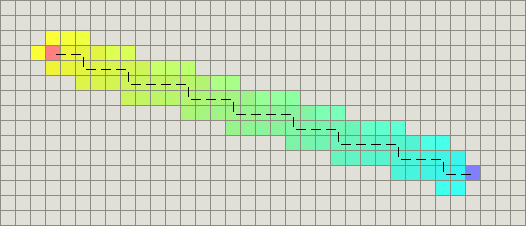
\includegraphics[scale=0.7]{manhattan.png}}
\caption{Манхэттенское расстояние}
\label{manh}
\end{figure}

\begin{figure}[h]
\center{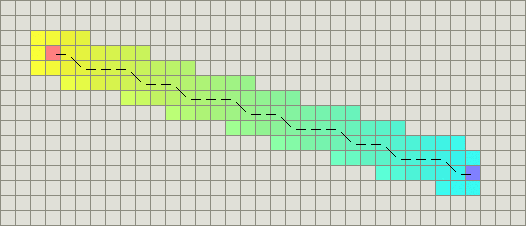
\includegraphics[scale=0.7]{diagonal.png}}
\caption{Диагональное расстояние}
\label{diag}
\end{figure}

\subsection{Реализация интерфейса}
\subsubsection{Внешняя спецификация}
Интерфейс программы представляет из себя 4 основных элемента: карта, панель управления, информационное окно, окно дополнительных настроек.

Карта (рис. \ref{map}) является главным элементом всего интерфейса, на ней выполняется демострация алгоритмов. По умолчанию размер каждой клетки равен 30 пикселям[], а количество клеток задаётся автоматически на основе размера экрана устройства. Выбор стартовой или конечной точки производится по клику.
Устанавливать или убирать препятствия можно не только по клику, но и при движении мыши с зажатой кнопкой. Если на клетке нет препятствия, то оно установится, в противном случае уберётся. После выполнения поиска путь нарисуется на карте линией. Если включен режим отладки (кнопка Debug), то обработанные клетки покроются голубым цветом

\begin{figure}[h]
\center{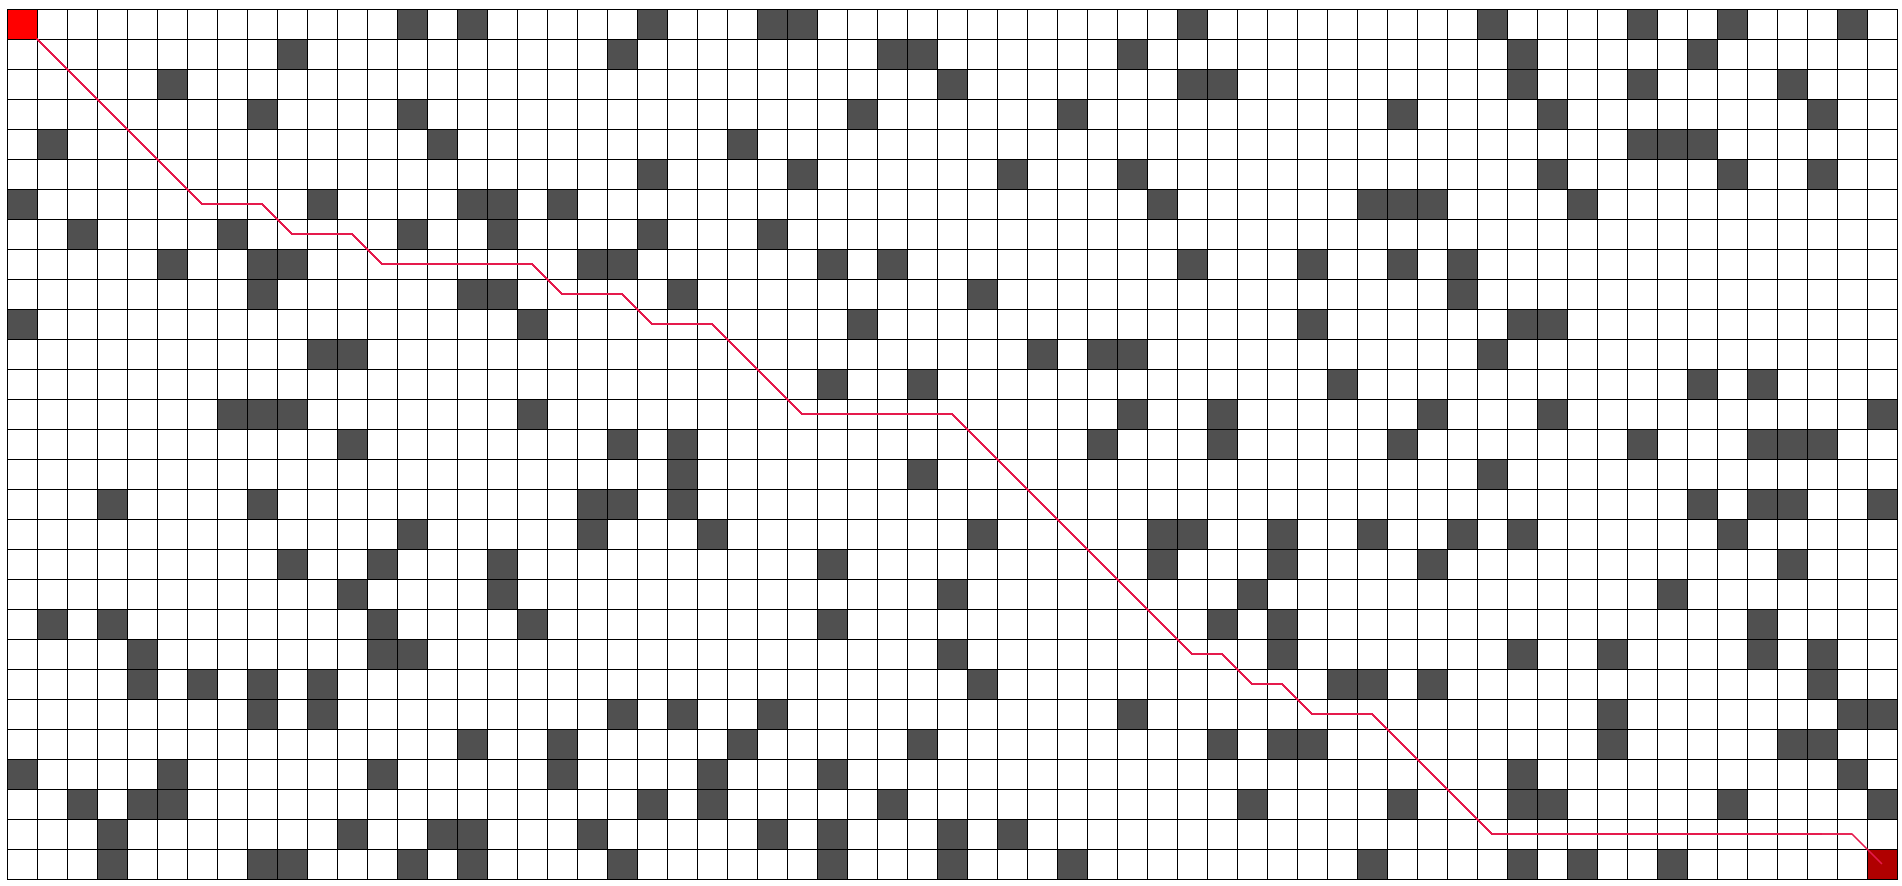
\includegraphics[scale=0.3]{map.png}}
\caption{Карта}
\label{map}
\end{figure}

В панели управления (рис. \ref{ctrlPanel}) можно изменить размеры карты, коэффциент случайной генерации препятствий (при 0 препятствий нет), включить режим отладки для просмотра обрабатываемых алгоритмом клеток, переключатся между режимом выбора конечной и стартовой точки и режимом установки препятствий, скрыть или показать окно информации, открыть окно дополнительных настроек.

\begin{figure}[h]
\center{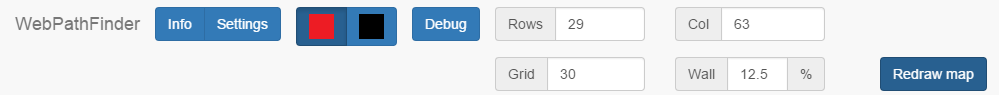
\includegraphics[scale=0.62]{cntlPanel.png}}
\caption{Панель управления}
\label{ctrlPanel}
\end{figure}

Информационное окно (рис. \ref{info}) привязано к кнопке Info и отображает информацию о последнем поиске пути: использованный алгоритм, время поиска, длину кратчайшего пути и количество обработанных клеток (при включенном режиме отладки). Если путь не удалось найти, то окно уведомит об этом.

\begin{figure}[h]
\center{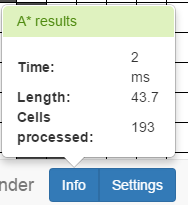
\includegraphics[scale=0.9]{info.png}}
\caption{Информационное окно}
\label{info}
\end{figure}

В окне дополнительных настроек (рис. \ref{sett}) можно сменить алгоритм поиска, настроить режим отладки (WIP), отключить отрисовку границ клеток (необходимо при задании больших карт с клетками в 1-2 пикселя), отключить диагональное движение.

\begin{figure}[h]
\center{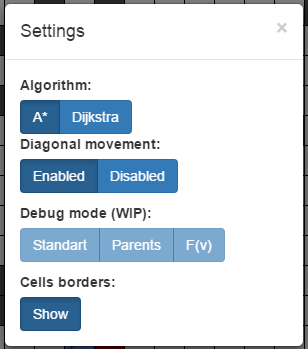
\includegraphics[scale=0.9]{sett.png}}
\caption{Дополнительные настройки}
\label{sett}
\end{figure}


\subsubsection{Внутренняя спецификация}
Интерфейс построен на обработчиках событий (англ. Event Handlers). При происхождении указанного события с указанным элементом интерфейса происходит вызов функции. Используются следующие события:

\begin{itemize}
\item Mousedown — срабатывает при нажатии кнопки мышки, наложен на слои карты (всего слоёв два: основной и слой для анимации). Определяет установку стартовой и конечной точки или стены.
\item Mousemove — срабатывает при движении мыши, наложен на основной слой карты. Определяет клетку, на которой находится курсор, и установку/удаление препятствий при движении мыши.
\item Click — срабатывает при клике на элемент. Наложен на кнопки. («Redraw map», «Settings»)
\item Change — срабатывает при кликах на checkbox и radiobox. Определяет изменение практически всех параметров для поиска.
\item Keydown — срабатывает при нажатии кнопки на клавиатуре. Наложен на все поля ввода и вызывает перерисовку карты при нажатии кнопки Enter.
\end{itemize}

Для отрисовки карты используется Canvas — элемент HTML5 предназначенный для создания изображения при помощи встроенных методов на JavaScript.

Анимации созданы с помощью методов Canvas и функций setTimeout и setInterval, которые выполняют код функции через указанное время. Язык JavaScript не имеет команды sleep. Анимации выполняются после окончания поиска пути и не отражают реальное время работы алгоритма. Искусственное замедление сделано для более понятной визуализации.

Поиск пути на больших картах занимает значительное время, в этот момент браузер полностью занят выполнением функции поиска и не обрабатывает интерфейс, что вызывает его зависание на время работы алгоритма. На маленьких картах этого не заметно.

